\documentclass[12pt]{article}
\usepackage[a4paper, margin=2.5cm]{geometry} % Indstiller margen til 2.5 cm
\usepackage{setspace} % Til linjeafstand
\onehalfspacing % Indstiller linjeafstand til 1.5
\usepackage{graphicx} % Til billeder
\usepackage{amsmath, amssymb} % Til matematiske udtryk
\usepackage{booktabs} % Til tabeller
\usepackage{caption} % Bedre kontrol over billedtekst
\usepackage{float} % Tillader placering af figurer på en ny side
\usepackage{pgfplots}
\usetikzlibrary{intersections, patterns, decorations.markings, calc}

\title{Macroeconomics III - Assignment 2}
\author{Emil Oliver Olesen (fps618) \& Carl-Emil Rohde (kvb125)}
\date{Apr 2026}

\begin{document}

\maketitle

\section{Exercise 1 - Business cycle empirics and costs}
\subsection{a)}

We use quarterly real series for GDP, consumption, and investment for the US (FRED: GDPC1, PCECC96, GPDIC1) and Portugal (Eurostat: \texttt{B1GQ}, \texttt{P3}, \texttt{P5G}, chain-linked volumes, seasonally and calendar adjusted). Each series is transformed to logs and filtered with an HP filter with $\lambda_{HP}=1600$.

\begin{figure}[H]
    \centering
    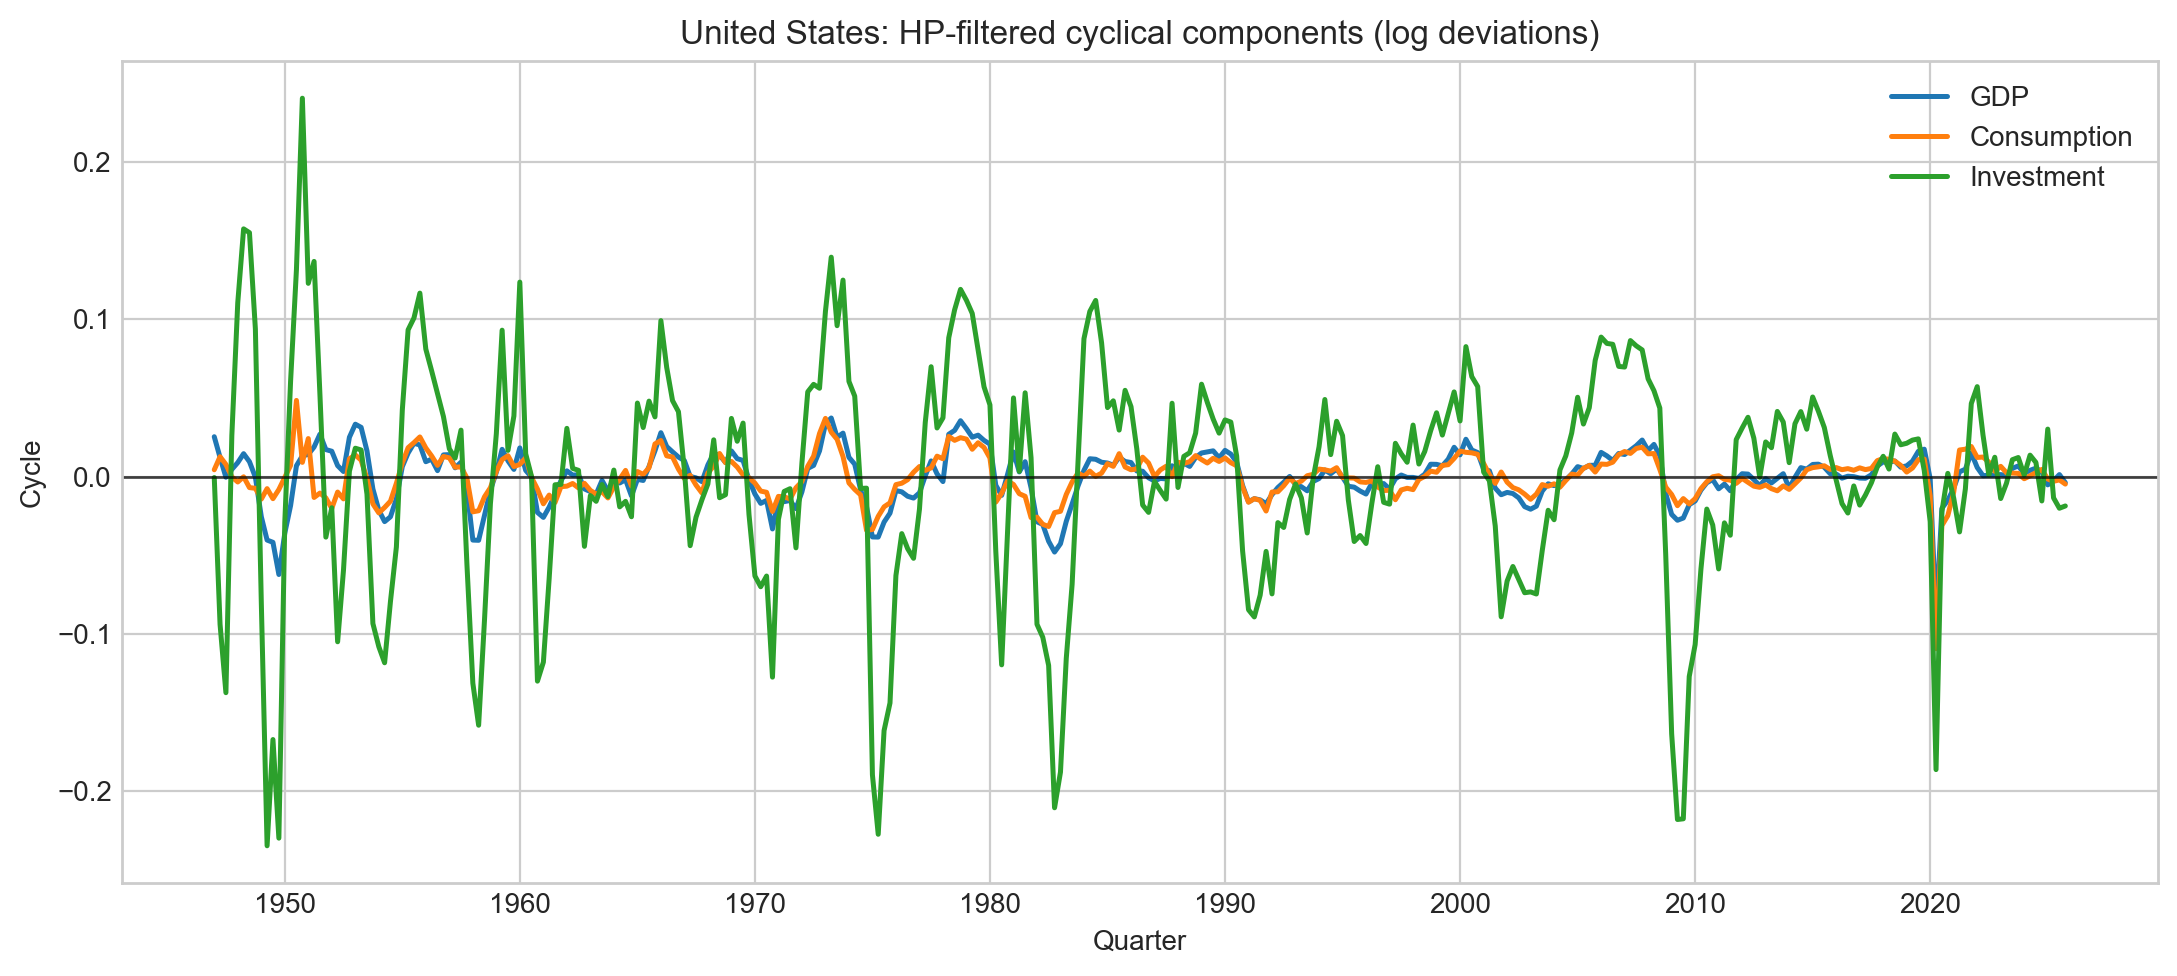
\includegraphics[width=0.92\linewidth]{fig_ex1a_us_cycles.png}
    \caption{US cyclical components from HP-filtered log GDP, consumption, and investment.}
    \label{fig:ex1a_us_cycles}
\end{figure}

\begin{figure}[H]
    \centering
    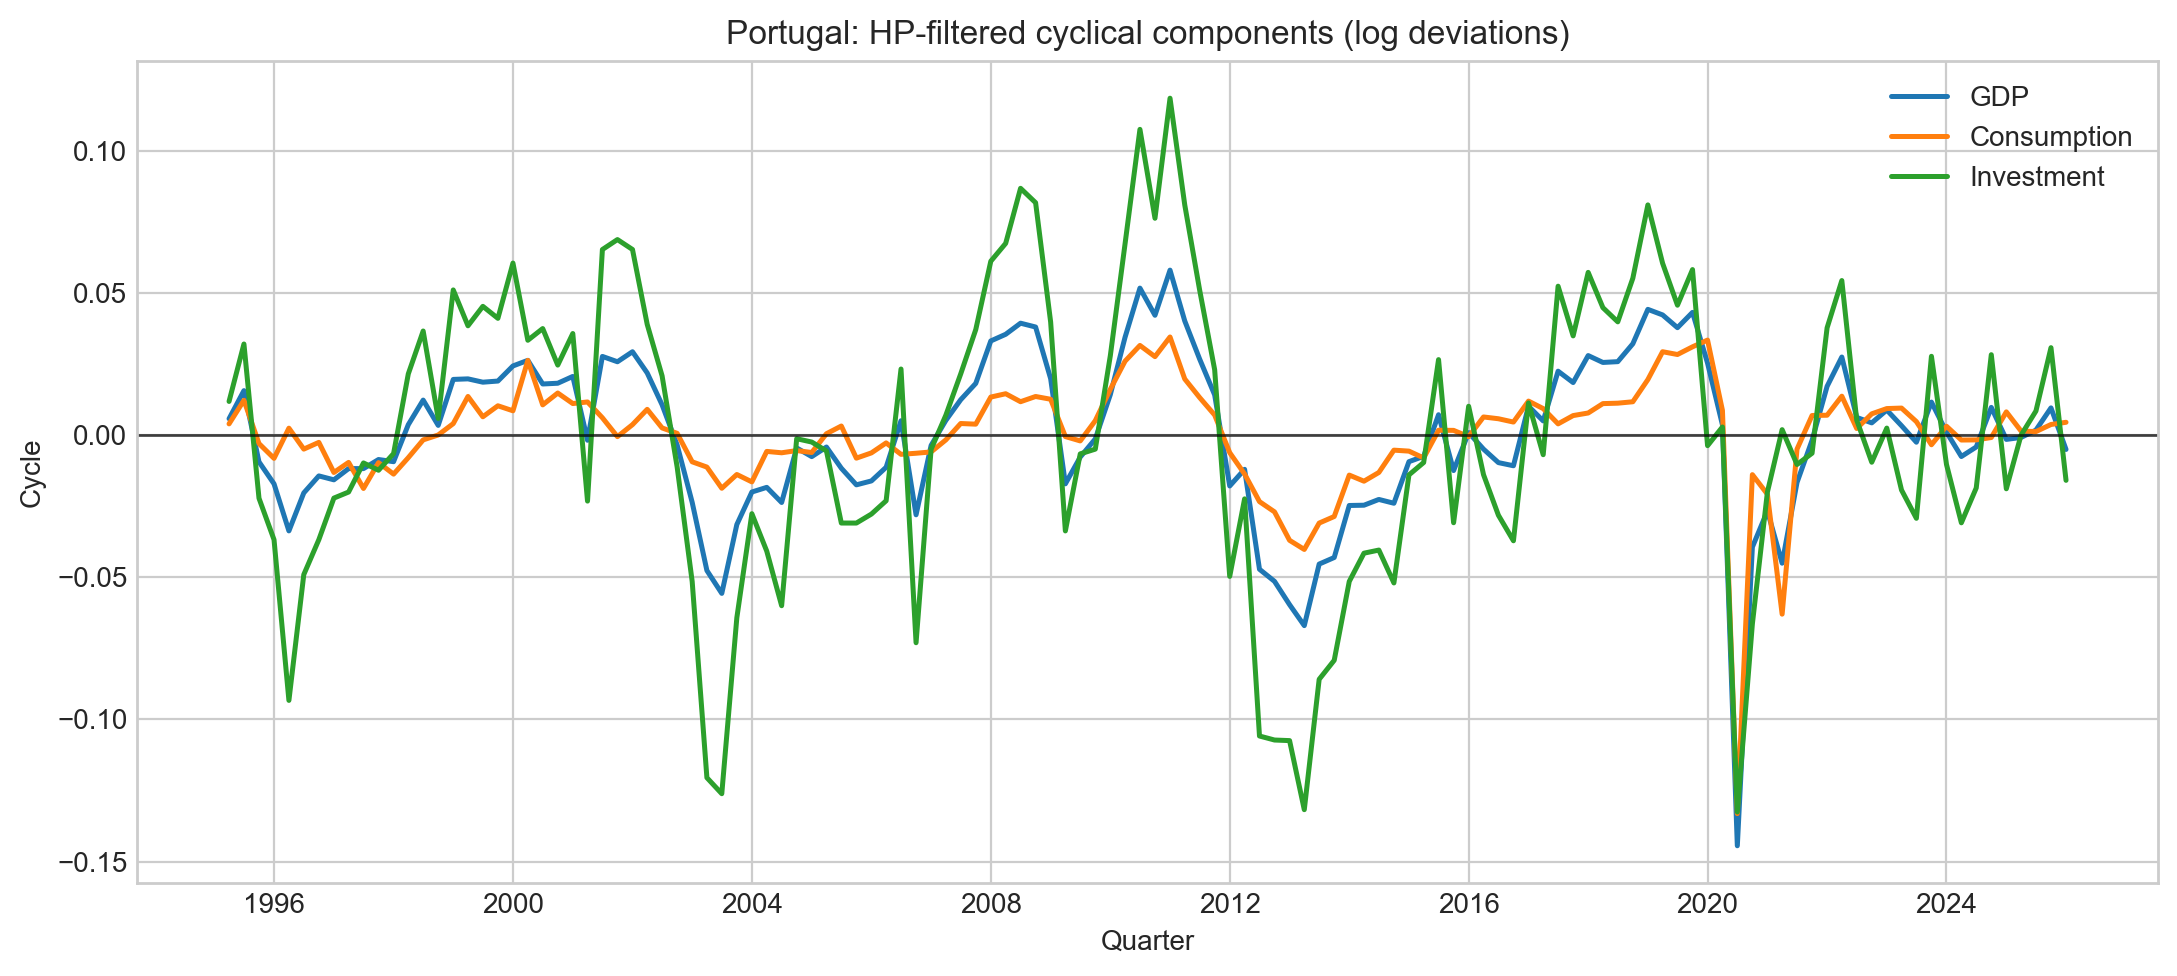
\includegraphics[width=0.92\linewidth]{fig_ex1a_pt_cycles.png}
    \caption{Portugal cyclical components from HP-filtered log GDP, consumption, and investment.}
    \label{fig:ex1a_pt_cycles}
\end{figure}

The figures show the standard pattern in both countries: investment is visibly the most volatile component, while consumption is smoother than output.

\subsection{b)}

Table \ref{tab:ex1b_vol} reports standard deviations of cyclical components and relative volatilities.

\begin{table}[H]
\centering
\caption{Business-cycle volatility moments}
\label{tab:ex1b_vol}
\begin{tabular}{lccccc}
\toprule
Country & $\sigma_y$ & $\sigma_c$ & $\sigma_i$ & $\sigma_c/\sigma_y$ & $\sigma_i/\sigma_y$ \\
\midrule
United States & 0.0162 & 0.0137 & 0.0708 & 0.8427 & 4.3592 \\
Portugal      & 0.0281 & 0.0191 & 0.0510 & 0.6799 & 1.8134 \\
\bottomrule
\end{tabular}
\end{table}

For both countries, $\sigma_c/\sigma_y<1$, so consumption is less volatile than output. Also, $\sigma_i/\sigma_y\gg 1$, so investment is much more volatile than output. Qualitatively, business cycles are similar across countries, although the US has markedly higher investment volatility relative to output, while Portugal has a larger output volatility level.

\subsection{c)}

Assume CRRA utility,
$$
u(c)=\frac{c^{1-\gamma}-1}{1-\gamma}, \quad \gamma=1.99.
$$
With normalized consumption $\tilde c_t=1+\varepsilon_t$ and $\varepsilon_t\sim U[-\varepsilon,\varepsilon]$, we match model volatility to the data via
$$
\sigma(\tilde c_t)=\frac{\varepsilon}{\sqrt{3}} \Rightarrow \varepsilon=\sqrt{3}\,\sigma_c.
$$
This gives $\varepsilon_{US}=0.023697$ and $\varepsilon_{PT}=0.033121$.

Using
$$
\mathbb{E}\left[(1+\varepsilon_t)^{1-\gamma}\right]
=\frac{1}{2\varepsilon}\frac{1}{2-\gamma}\left[(1+\varepsilon)^{2-\gamma}-(1-\varepsilon)^{2-\gamma}\right],
$$
we obtain:
\begin{table}[H]
\centering
\caption{Welfare comparison for $\gamma=1.99$}
\label{tab:ex1c}
\begin{tabular}{lccc}
\toprule
Country & $\sigma_c$ & $\varepsilon$ & $\mathbb{E}[(1+\varepsilon_t)^{1-\gamma}]$ \\
\midrule
United States & 0.013681 & 0.023697 & 1.000184 \\
Portugal      & 0.019122 & 0.033121 & 1.000360 \\
\bottomrule
\end{tabular}
\end{table}

The compensating variation that makes the agent indifferent between US and Portuguese risk is
$$
\lambda_{US\to PT}=-0.000178 \;(-0.0178\%), \qquad
\lambda_{PT\to US}=+0.000178 \;(0.0178\%).
$$
Interpretation: Portuguese aggregate consumption risk is higher in this sample, but the implied welfare gap is very small (around two-hundredths of one percent of consumption).

\subsection{d)}

Recomputing with $\gamma=4$ (same empirical $\sigma_c$ and therefore same $\varepsilon$):
$$
\lambda_{US\to PT}=-0.000357 \;(-0.0357\%), \qquad
\lambda_{PT\to US}=+0.000357 \;(0.0357\%).
$$
So $|\lambda|$ is larger than in part (c). This is expected: higher risk aversion implies a larger welfare cost of a given amount of consumption risk.

\subsection{e)}

Now compare economy (a) with economy (c), where each period:
$$
c_h=1.02\bar c \text{ with probability }0.95, \qquad
c_l=0.62\bar c \text{ with probability }0.05,
$$
and set $\gamma=2$.

Because part (a) was estimated for two countries, economy (a) has two empirical calibrations:
\begin{table}[H]
\centering
\caption{Indifference $\lambda$ between economy (a) and economy (c), $\gamma=2$}
\label{tab:ex1e}
\begin{tabular}{lccc}
\toprule
Economy (a) calibration & $\mathbb{E}_a$ & $\mathbb{E}_c$ & $\lambda_{a\to c}$ \\
\midrule
US $\sigma_c$ calibration & 1.000187 & 1.012018 & -0.011690 \;(-1.169\%) \\
Portugal $\sigma_c$ calibration & 1.000366 & 1.012018 & -0.011513 \;(-1.151\%) \\
\bottomrule
\end{tabular}
\end{table}

The negative sign means economy (a) is preferred: the individual would accept about a 1.15--1.17\% reduction in consumption in economy (a) and still be indifferent to economy (c). This is much larger than the representative-agent aggregate business-cycle costs above (around 0.02--0.04\%), so business cycles are not ``costless'' once large idiosyncratic downside risk (such as unemployment risk) is introduced.


\section{Exercise 2}
\subsection{a)}
We have the matching function, which tells us the total number of matches formed in a period. We want to turn that into probabilities for each side of the market.
\paragraph{Job-finding probability}
this means finding out of all the matches formed, what fraction of the unemployed pool gets matched?
$$
f(\theta)=\frac{M(u, v)}{u}
$$
Plugging in the matching function:
$$
f(\theta)=\frac{u^\gamma v^{1-\gamma}}{u}=u^{\gamma-1} v^{1-\gamma}
$$
Rewrite everything in terms of $\theta=\mathrm{v} / \mathrm{u}$:
$$
f(\theta)=u^{\gamma-1} \cdot v^{1-\gamma}=u^{\gamma-1} \cdot u^{1-\gamma} \cdot\left(\frac{v}{u}\right)^{1-\gamma}
$$
reduce:
$$
\boxed{f(\theta)=\theta^{1-\gamma}}
$$
The intuituin is when the market is tight, hight $\theta$ $\rightarrow$ lots of vacancies per unemployed $\rightarrow$ workers find jobs more easily $\rightarrow$ f is increasing in $\theta$.
\paragraph{Vacancy-filling probability}
Same logic, but from the firm's side. Out of all matches formed, what fraction of vacancies gets filled?
$$
\eta(\theta)=\frac{M(u, v)}{v}
$$
Plugging in:
$$
\eta(\theta)=\frac{u^\gamma v^{1-\gamma}}{v}=u^\gamma v^{-\gamma}
$$
Again, rewrite
$$
\eta(\theta)=\left(\frac{u}{v}\right)^\gamma=\left(\frac{v}{u}\right)^{-\gamma}
$$
$$\boxed{\eta(\theta)=\theta^{-\gamma}}$$
Intuituin here is when the market is tight ( $\theta$ high), there are many vacancies chasing few workers, so each individual firm has a harder time filling its vacancy $-\eta$ is decreasing in $\theta$.

\subsection{b)}
In steady state the inflow into unemployment and outflow out of unemployment must balance:
$$
\delta(1-u)=f(\theta) \cdot u
$$
Now we solve for $u$:
$$
\delta-\delta u=f(\theta) \cdot u
$$
Collect the $u$ terms on one side:
$$
\delta=f(\theta) \cdot u+\delta u=u[f(\theta)+\delta]
$$

$$\boxed{u=\frac{\delta}{\delta+f(\theta)}}$$
\textbf{Intuition: }Unemployment is high when separations $\delta$ are large and low when $\mathrm{f}(\theta)$ is large. It's just the ratio of the inflow rate to the total turnover rate.

\subsubsection{Drawingt the Beveridge curve}
Since $\theta=\mathrm{v} / \mathrm{u}$, we can substitute back:
$$
u=\frac{\delta}{\delta+f(v / u)}
$$
This defines a curve in (u, v) space, namely the beveridge curve:
\begin{figure}[H]
    \centering
    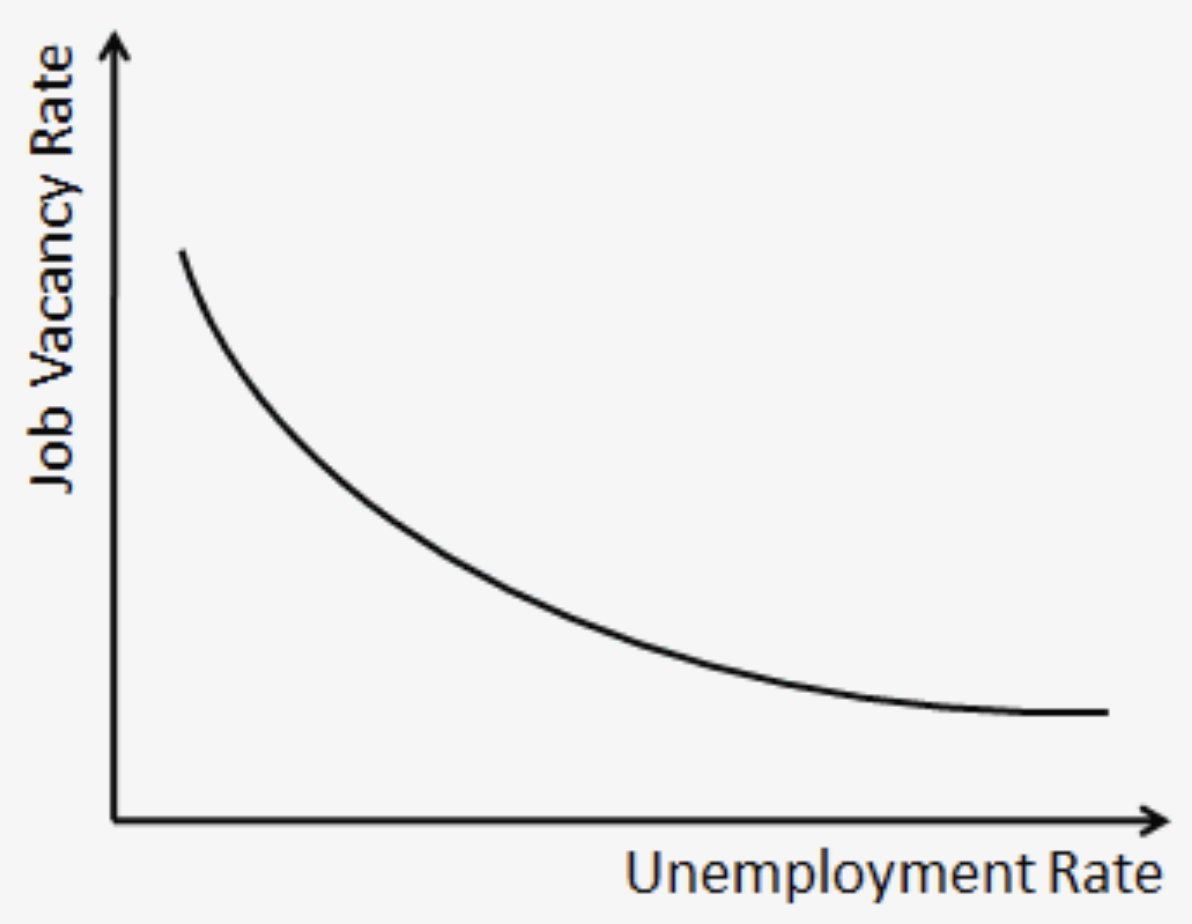
\includegraphics[width=0.5\linewidth]{curve.png}
    \caption{The beveridge curve    }
    \label{fig:placeholder}
\end{figure}
Unemployment and vacancies are negatively related along this curve. When vacancies are high, workers find jobs quickly and unemployment is low. When vacancies are scarce, job finding is slow and unemployment piles up. 

\end{document}